\documentclass{beamer}
\usetheme{metropolis}
\usepackage{graphicx}
\usepackage{subfig}
\usepackage{hyperref}
\usepackage{tcolorbox}
\title{Algebra-Based Physics-1: Mechanics (PHYS135A-01): Week 4}
\date{September 25th - September 29th, 2017}
\author{Jordan Hanson}
\institute{Whittier College Department of Physics and Astronomy}

\begin{document}
\maketitle

\section{Week 3 Review}

\begin{frame}{Week 3 Review}
\begin{enumerate}
\item Working with vectors: displacement, velocity and acceleration
\begin{itemize}
\item Breaking into components, graphical methods
\item Analytical methods
\item \textbf{Lab-activity: measuring different accelerations}
\item \textbf{Lab-activity: testing component independence}
\end{itemize}
\item Combining free-fall and vector components: \alert{projectile motion}
\item Relative motion and addition of velocities
\end{enumerate}
\end{frame}

\section{Week 3 Review Problems}

\begin{frame}{Week 3 Review Problems}
\small
A pilot is performing an airdrop maneuver, in which he must release a package of supplies to land on a beach.  The plane is traveling towards the beach at a speed of 100 kilometers per hour, with an altitude of 500 meters.  How far offshore must the pilot release the supplies such that the package lands on the sandy beach and not in the water?
\begin{itemize}
\item A: 280 m 
\item B: 410 m
\item C: 100 m
\item D: 170 m
\end{itemize}
\end{frame}

\begin{frame}{Week 3 Review Problems}
\small
Suppose the pilot is flying straight, adjusting for a cross-wind of 3 m/s.  How far to the side of the flight path of the plane does the package land, assuming the package is released 280 m from the shore?
\begin{itemize}
\item A: 10 m
\item B: 20 m
\item C: 30 m
\item D: 40 m
\end{itemize}
\end{frame}

\section{Week 4 Summary}

\begin{frame}{Week 4 Summary}
\begin{figure}
\centering
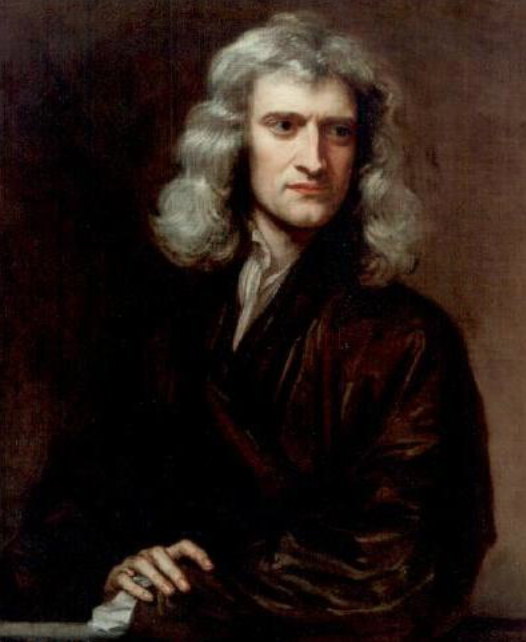
\includegraphics[width=0.5\textwidth]{figures/newton.png}
\caption{\label{fig:newton} A portrait of Sir Isaac Newton.}
\end{figure}
\end{frame}

\begin{frame}{Week 4 Summary}
\begin{enumerate}
\item Deep statements about physics: \textit{dynamics} and \textit{kinematics}
\begin{itemize}
\item \textbf{Lab activity}: Force, mass and stretching springs
\end{itemize}
\item Newton's \alert{First Law}
\begin{itemize}
\item \textbf{Lab activity}: force tables
\end{itemize}
\item Newton's \alert{Second Law}
\item Newton's \alert{Third Law}
\item Applications
\begin{itemize}
\item Free-body diagrams
\item Tension
\item Inclined surfaces
\item Restoring forces
\end{itemize}
\end{enumerate}
\end{frame}

\begin{frame}{Deep statements about physics: dynamics and kinematics}
\small
\textit{Kinematics} - A \alert{description} of the motion of particles and systems \\
\textit{Dynamics} - An \alert{explanation} of the motion of particles and systems \\
\vspace{0.25cm}
What causes an object to move?  \textbf{Forces}.  Forces exist as a result of the \alert{\textbf{interactions}} of objects or systems.\\
\vspace{0.25cm}
\rule{10cm}{0.4pt} \\
\vspace{0.25cm}
\textit{Evolution} - A \alert{description} of the change of biological species \\
\textit{Natural Selection} - An \alert{explanation} of change in biological species \\
\vspace{0.25cm}
What causes species to evolve?  \textbf{Natural selection}.  Natural selection exists because of \alert{election pressures}, \alert{numerous offspring}, and \alert{variation} among offspring.
\end{frame}

\begin{frame}{What is a force, in practice?}
A force has units of \textit{Newtons}, just like distance has units of \textit{meters}.  One Newton is the force required to make an object of mass 1 kilogram accelerate by 1 m/s$^2$.\\
\vspace{1cm}
A force must also be a \textit{vector}: if a force acts on a system in a certain direction, the object will accelerate in that direction. \\
\vspace{1cm}
Force has to be related to mass in some way.
\end{frame}

\begin{frame}{What is a force, in practice?}
\small
\begin{figure}
\centering
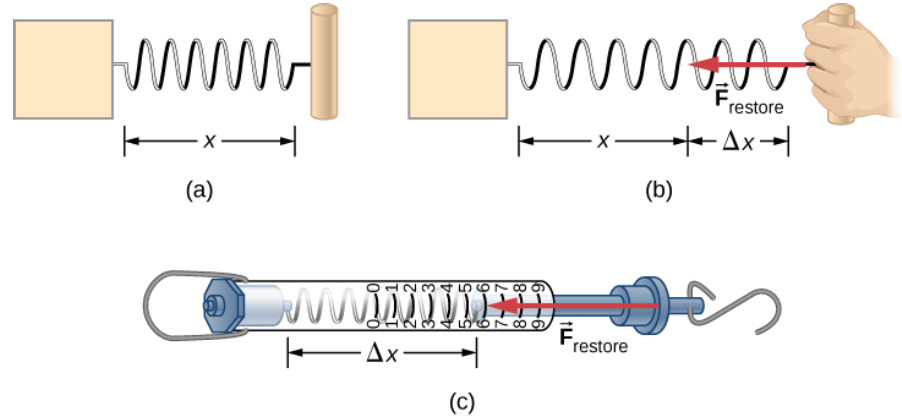
\includegraphics[width=0.9\textwidth]{figures/force1.png}
\caption{\label{fig:force1} (a) No interaction is stretching the spring.  (b) An interaction stretches the spring a distance $\Delta x$, and the spring pulls back.  (c) A device that can compare forces by comparing $\Delta x$ for different interactions (connecting to different weights, for example).}
\end{figure}
\end{frame}

\begin{frame}{What is a force, in practice?}
\textbf{Lab activity}: Force, mass, and stretched springs.
\begin{enumerate}
\item Obtain a set of weights, a force-meter (spring), and a ruler.
\item Hang a weight from the spring, and measure the extra distance the spring stretches.
\item Repeat with different weights, recording the stretched distances alongside the weights.
\item Compute the ratio of the mass of the weight to the stretched distance in each case.  What is the result?
\end{enumerate}
\end{frame}

\begin{frame}{What is a force, in practice?}
Thus, if a force causes \textit{a system with some mass} to accelerate, the force must be \textit{proportional to that mass}.  \alert{``If it is heavier, we mush push it harder, to obtain the same acceleration.''}  \\
\vspace{1cm}
Now, let's consider all the systems for which we have described the \textit{kinematics}, where we made no use of the concept of a force...
\end{frame}

\section{Newton's First Law}

\begin{frame}{Newton's First Law}
\begin{tcolorbox}[colback=white,colframe=red!40!blue,title=Newton's First Law]
\alert{A body at rest remains at rest or, if in motion, remains in motion at constant velocity unless acted on by a net external force.}
\end{tcolorbox}
\end{frame}

\begin{frame}{Newton's First Law}
\small
For most people in the late 15th and early 16th centuries, Newton's First Law was not intuitive.  ``When have you ever seen a thing move perpetually?''\\
\vspace{0.5cm}
The key is the last phrase: ``\textit{...unless acted on by a \alert{net} external force}.''  Nothing moves unless forced, and if the \alert{net} force is zero, the velocity does not change.  Thus, if some object has a constant velocity, then it remains at that velocity unless some force (friction, air-resistance, gravity, a wall) interrupts. \\
\vspace{0.5cm}
\url{https://openstaxcollege.org/l/21forcemotion} \\
Write down your observations about the net force on the object.
\end{frame}

\begin{frame}{Newton's First Law}
\small
\textbf{Lab activity}: Force tables
\begin{enumerate}
\item Obtain a set of weights, and a force-table, with ring and pulley system.
\item Using knowledge of vectors, arrange weights on the pulleys such that the ring remains stationary in the center.
\item Double one of the weights, and find the angles the strings must make to keep the ring stationary in the center.
\item Define the force vectors as vectors with magnitudes equal to the masses of the weights, in the directions of the strings.  Do the vectors add to zero?
\item Why does the ring remain stationary even though there are three forces from strings acting on it?
\end{enumerate}
\end{frame}

\begin{frame}{Newton's First Law}
\begin{figure}
\centering
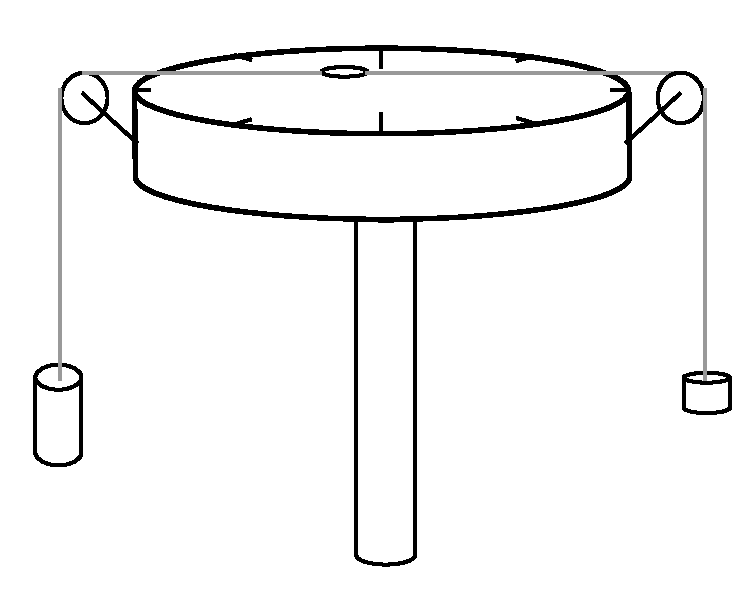
\includegraphics[width=0.6\textwidth]{figures/Table.pdf}
\caption{\label{fig:table} The force table setup includes a wheel with angles, strings and pulleys, and a central ring.}
\end{figure}
\end{frame}

\begin{frame}{Newton's First Law}
Newton's First Law may be thought of in terms of the following equation:
\begin{equation}
\boxed{F_{\rm net} = \sum_{\rm i} \vec{F}_{\rm i} = 0}
\label{eq:firstlaw}
\end{equation}
In the case of the force table ring, $\vec{F}_{\rm i} \neq 0$ but $\vec{F}_{\rm net} = 0$, so we observe no velocity.  We can also have a situation with constant velocity and $\vec{F}_{\rm net} = 0$  but $\vec{F}_{\rm i} \neq 0$.
\end{frame}

\begin{frame}{Newton's First Law}
A man slides a palette crate across a concrete floor of his shop.  He exerts a force of 60.0 N, and the box has a constant velocity of 0.5 m/s.  What force cancels his pushing force, and what is the magnitude of that force?
\begin{itemize}
\item A: wind, 60.0 N
\item B: friction: 60.0 N
\item C: friction: -60.0 N
\item D: weight: -60.0 N
\end{itemize}
\end{frame}

\begin{frame}{Newton's First Law}
\small
\textit{Newton's First Law and Inertial Reference Frames}.  If an object has a constant velocity in one frame of reference, it has a constant velocity in another frame of reference moving at a constant velocity with respect to the first frame.  Consider the prior problem, and a second man is walking in the opposite direction as the palette crate at a speed of 1 m/s.  What is the speed of the palette crate from his perspective?  What is the first man's force on the palette crate from his perspective?
\begin{itemize}
\item A: 1.5 m/s, 60.0 N
\item B: 1.5 m/s, -60.0 N
\item C: 0.5 m/s, 0.0 N 
\item D: -1.5 m/s, -60.0 N
\end{itemize}
\end{frame}

\section{Newton's Second Law}

\begin{frame}{Newton's Second Law}
From the prior problem, we see that \alert{Newton's First Law} holds even under relativity, for inertial reference frames.  Let's assume we observe a system from an intertial reference frame. \\
\vspace{0.5cm}
Let us also ignore any \textit{internal forces}: forces components of the system apply to each other.  Focusing on the external forces only, we make the following two observations: \\
\end{frame}

\begin{frame}{Newton's Second Law}
\begin{figure}
\centering
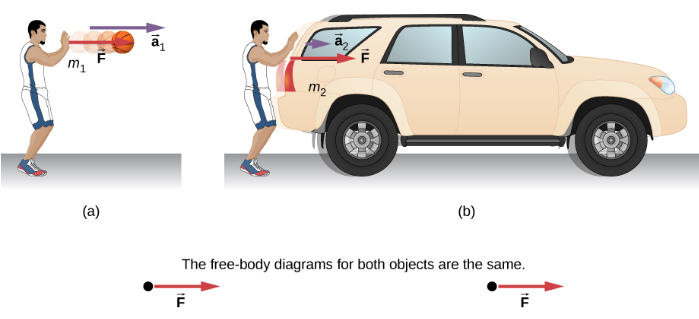
\includegraphics[width=0.9\textwidth]{figures/NewtonsSecond.png}
\caption{\label{fig:newton1} A force produces greater acceleration for less massive objects.}
\end{figure}
\end{frame}

\begin{frame}{Newton's Second Law}
\begin{figure}
\centering
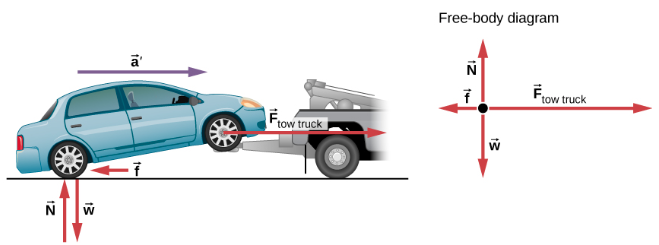
\includegraphics[width=0.9\textwidth]{figures/NewtonsSecond2.png}
\caption{\label{fig:newton2} A larger force produces greater acceleration for a given mass.}
\end{figure}
\end{frame}

\begin{frame}{Newton's Second Law}
\begin{tcolorbox}[colback=white,colframe=red!40!blue,title=Newton's Second Law]
\alert{The net force on a system is equal to the mass of the system multiplied by the acceleration of the system: $\vec{F}_{\rm net} = m \vec{a}$}
\end{tcolorbox}
\end{frame}

\begin{frame}{Newton's Second Law}
A man slides a palette crate across a concrete floor of his shop.  He exerts a force of 60.0 N, and friction pushes against the crate with a force of 40.0 N.  What is the acceleration of the crate, if the crate is loaded with 50.0 kg of material?
\begin{itemize}
\item A: 0.1 m/s$^2$
\item B: 1.0 m/s$^2$
\item C: 0.5 m/s$^2$
\item D: 0.4 m/s$^2$
\end{itemize}
\end{frame}

\begin{frame}{Newton's Second Law}
A man slides a palette crate across a concrete floor of his shop.  He exerts a net force of 30.0 N, and the crate accelerates at 0.5 m/s$^2$.  What mass is loaded onto the crate?
\begin{itemize}
\item A: 40.0 kg
\item B: 50.0 kg
\item C: 60.0 kg
\item D: 70.0 kg
\end{itemize}
\end{frame}

\begin{frame}{Newton's Second Law}
\begin{figure}
\centering
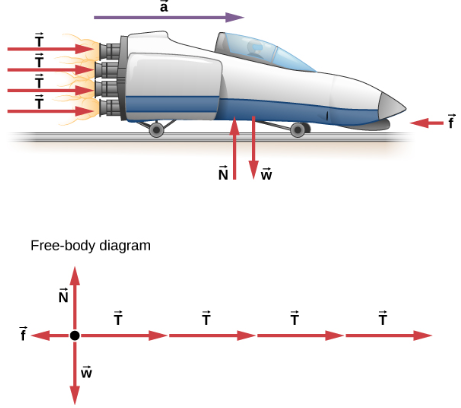
\includegraphics[width=0.5\textwidth]{figures/NewtonsSecond3.png}
\caption{\label{fig:newton3} An example of a \textit{free body diagram}, which summarizes all external forces on a system.}
\end{figure}
\end{frame}

\begin{frame}{Newton's Second Law}
\begin{figure}
\centering
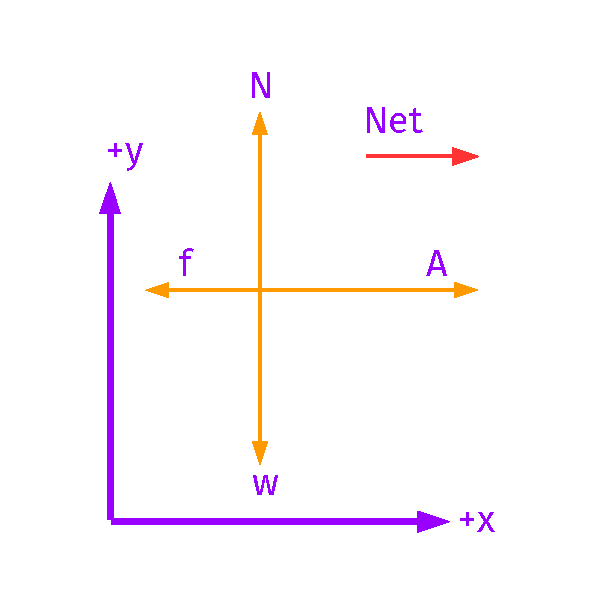
\includegraphics[width=0.5\textwidth,trim=0.75cm 0.5cm 0.75cm 0.5cm,clip=true]{figures/NetForce.pdf}
\caption{\label{fig:fbd} The \textit{free-body diagram} is just a vector summation problem.  The \textit{normal force}, \textbf{N}, acts against the force of gravity, \textbf{w}, according to Netwon's Third Law.}
\end{figure}
\end{frame}

\begin{frame}{Newton's Second Law}
Indiana Jones is running through the rainforest, and he wades into a pit of quicksand.  He has a mass of 70 kg, however the normal force is only 400.0 N.  He pushes forward with a force of 250.0 N, and the quicksand sucks him backwards with a force of 50.0 N.  What is the net force on Indiana?  The force of gravity is his mass times $g$, in the downward direction.
\begin{itemize}
\item A: (200.0, -290) N
\item B: (50.0, -690) N
\item C: (200.0, 290) N
\item D: (150.0, 690) N
\end{itemize}
\end{frame}

\begin{frame}{Newton's Second Law}
What is the magnitude of the net acceleration on Indiana, from the previous example?
\begin{itemize}
\item A: 1.0 m/s$^2$
\item B: 3.0 m/s$^2$
\item C: 4.0 m/s$^2$
\item D: 5.0 m/s$^2$
\end{itemize}
\end{frame}

\begin{frame}{Newton's Second Law}
A bit of mathematics: \alert{notice that if we define $\vec{p} = m\vec{v}$}, we may write \\
\vspace{0.5cm}
\begin{equation}
\vec{F}_{\rm net} = \Delta\vec{p} = \Delta(m)\vec{v} + m\Delta(\vec{v}) = m \vec{a}_{\rm net}
\end{equation} \\
\vspace{0.5cm}
For systems with consant mass: force is the change in \textit{momentum}, $\vec{p}$.
\end{frame}

\begin{frame}{Newton's Second Law}
There is a difference between \alert{\textit{mass}}, and \alert{\textit{weight}}.  \textit{Mass} is proportional to the number of atoms in an object.  \textit{Weight} is a force derived from Newton's second law (mass times acceleration), assuming the acceleration due to gravity is constant.  If an object has a mass of 1 kilogram, and the Earth's gravitational acceleration is $\approx 10$ m/s$^2$, then it \textit{weighs} $\approx 10.0$ N (10.0 kg m/s$^2$).
\end{frame}

\begin{frame}{Newton's Second Law}
Astronauts are walking on the moon, and lifting moon rocks into cannisters.  On Earth, the cannisters weighed 40.0 N each, and each astronaut is expected to carry two of them, loaded each with 65.0 kg of moon rock.  The acceleration due to gravity on the Moon is about 17\% of that on Earth.  What weight are these astronauts expected to carry?
\begin{itemize}
\item A: 230 N
\item B: 200 N
\item C: 1000 N
\item D: 170 N
\end{itemize}
\end{frame}

\begin{frame}{Newton's Second Law}
Speaking of the Moon... \\
\vspace{1cm}
\url{https://phet.colorado.edu/en/simulation/legacy/lunar-lander} \\
\vspace{1cm}
For this demonstration, you may need to update Java.  Write down observations regarding:
\begin{itemize}
\item Difference between weight and mass
\item Balance of gravity and thrust
\item Changing mass of the system
\item Independence of vertical and horizontal motion
\end{itemize}
\end{frame}

\begin{frame}{Newton's Second Law}
Orbits...We will come back to this topic in Chapter 13. \\
\vspace{1 cm}
\url{https://phet.colorado.edu/en/simulation/gravity-and-orbits} \\
\vspace{1 cm}
For this demonstration, you may need to update Java.  Write down observations regarding:
\begin{itemize}
\item The effect of removing gravity on the orbits: what happens to velocities?
\item The effect of increasing the force of gravity (higher masses): what happens to orbits?
\end{itemize}
\end{frame}

\begin{frame}{Newton's Second Law}
A 20,000 kg jet fighter lands on an aircraft carrier, moving at 108 km/hr.  A tow cable grabs the aircraft and pulls it to a stop in 100 meters.  What is the average acceleration?  What force does the tow cable extert to stop the jet?
\begin{itemize}
\item A: 9.0 m/s$^2$, 90,000 N
\item B: 4.5 m/s$^2$, 90,000 N
\item C: 1.5 m/s$^2$, 45,000 N
\item D: 9.0 m/s$^2$, 45,000 N
\end{itemize}
\end{frame}

\section{Newton's Third Law}

\begin{frame}{Newton's Third Law}
\begin{tcolorbox}[colback=white,colframe=red!40!blue,title=Newton's Third Law]
\alert{Whenever one system, A, exerts a force on a second system, B, the first body experiences a force that is equal in magnitude and opposite in direction to the force that it exerts.
\begin{equation}
\vec{F}_{\rm AB} = -\vec{F}_{\rm BA}
\end{equation}}
\end{tcolorbox}
For every action, there is an equal and opposite reaction.
\end{frame}

\begin{frame}{Newton's Third Law}
\begin{figure}
\centering
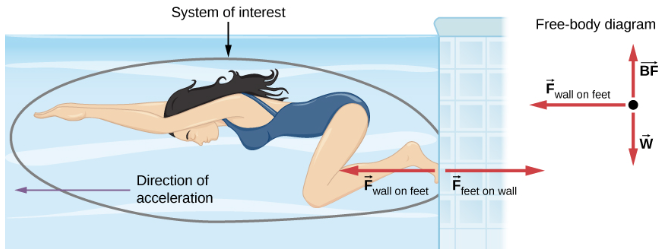
\includegraphics[width=0.9\textwidth]{figures/newtonsthird1.png}
\caption{\label{fig:newtons3} Defining the system properly is key to understanding Newton's Third Law.}
\end{figure}
\end{frame}

\begin{frame}{Newton's Third Law}
As mentioned before, the \textit{weight} of an object is $\vec{w} = -mg\hat{y}$, where $g$ is the acceleration due to gravity, pointing in the $-\hat{y}$ direction.  A stack of three books rests on a table.  Each book weighs 12.0 N.  If the books are not moving, what force is the table exerting on the books, from Newton's third law?
\begin{itemize}
\item A: 24.0 N
\item B: -24.0 N
\item C: -36.0 N
\item D: 36.0 N
\end{itemize}
\end{frame}

\begin{frame}{Newton's Third Law}
When Newton's third law indicates that the weight of an object is couterbalanced by a surface, we call the counterbalancing force the \alert{normal force}: $\vec{N} = mg\hat{y}$.  What is the normal force exterted by the middle book in the stack?  What is the normal force extered by the bottom book?
\begin{itemize}
\item A: 12.0 N, 24.0 N
\item B: 12.0 N, 12.0 N
\item C: 36.0 N, 24.0 N
\item D: 24.0 N, 12.0 N
\end{itemize}
\end{frame}

\section{Free Body Diagrams and Common Forces}

\begin{frame}{Free Body Diagrams and Common Forces}
\begin{figure}
\centering
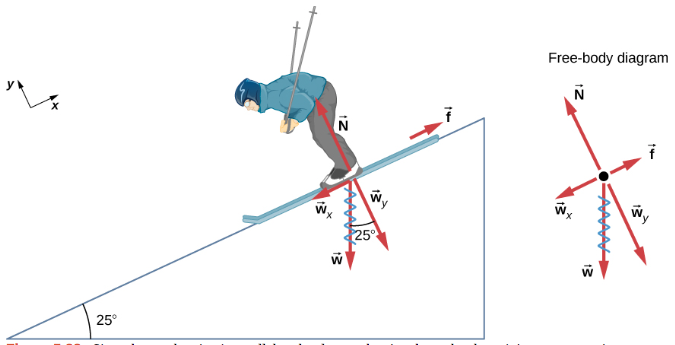
\includegraphics[width=0.8\textwidth,trim=0cm 0.1cm 0cm 0cm,clip=true]{figures/incline.png}
\caption{\label{fig:incline} In this example, the normal force counterbalances the weight of the system normal to the surface, but the weight is not along $\hat{y}$ exclusively.  The weight is must be broken into components, and Newton's third law provides the opposite of each.}
\end{figure}
\end{frame}

\begin{frame}{Free Body Diagrams and Common Forces}
\begin{figure}
\centering
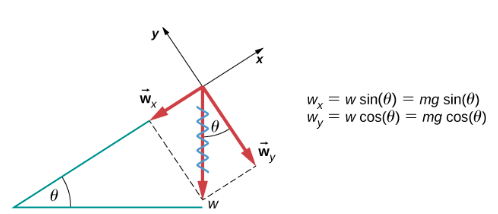
\includegraphics[width=0.9\textwidth]{figures/incline2.png}
\caption{\label{fig:incline2} A general description of forces on an incline.  Notice two things: 1) take the limit of $\theta = 0^{\circ}$ and $\theta = 90^{\circ}$, and 2) calculate $(w_x^2+w_y^2)^{1/2}$.}
\end{figure}
\end{frame}

\begin{frame}{Free Body Diagrams and Common Forces}
Using the previous diagram, calculate the force and acceleration of a 10 gram marble down the incline, if the incline is 45 degrees (let $g = 10$ m/s$^2$).
\begin{itemize}
\item A: $\frac{0.5}{\sqrt{2}}$ N, $-\frac{50}{\sqrt{2}}$ m/s$^2$
\item B: $\frac{10}{\sqrt{2}}$ N, $-\frac{10}{\sqrt{2}}$ m/s$^2$
\item C: $\frac{0.1}{\sqrt{2}}$ N, $\frac{10}{\sqrt{2}}$ m/s$^2$
\item D: $-\frac{0.1}{\sqrt{2}}$ N, $-\frac{10}{\sqrt{2}}$ m/s$^2$
\end{itemize}
\end{frame}

\begin{frame}{Free Body Diagrams and Common Forces}
Same system: what is the normal force exerted on the marble by the incline?
\begin{itemize}
\item A: $0.1/\sqrt{2}$ N
\item B: $1/\sqrt{2}$ N
\item C: $0.01/\sqrt{2}$ N
\item D: $0.1$ N
\end{itemize}
\textit{Why is the answer not just the value of $mg$?}
\end{frame}

\begin{frame}{Free Body Diagrams and Common Forces}
\small
Two more example forces: \textbf{\alert{tension}}, and the \textbf{\alert{spring force}}.  Tension is the force found in pulling an object.
\begin{figure}
\centering
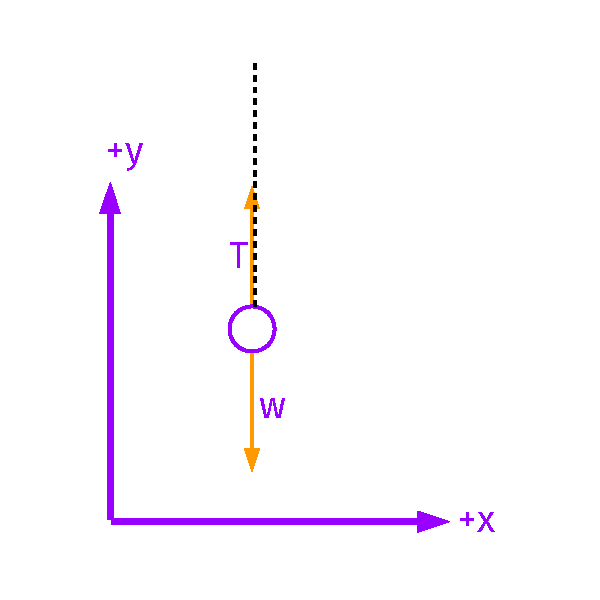
\includegraphics[width=0.4\textwidth]{figures/pend.pdf}
\caption{\label{fig:pend}  Consider a stationary pendelum of weight -2.0 N, hanging by a string.  The tension in the string must be 2.0 N, by Newton's third law.}
\end{figure}
\end{frame}

\begin{frame}{Free Body Diagrams and Common Forces}
\begin{figure}
\centering
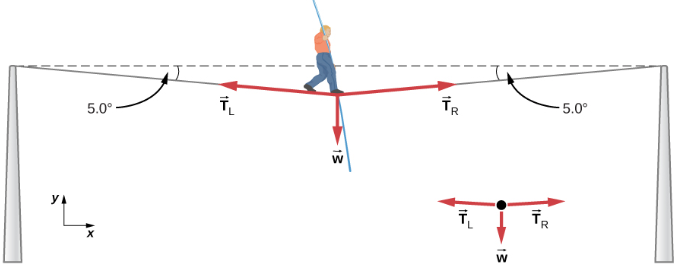
\includegraphics[width=0.8\textwidth]{figures/tightrope.png}
\caption{\label{fig:tightrope} Tension in the tightrope balances the weight of the system, but there is additional tension.}
\end{figure}
\end{frame}

\begin{frame}{Free Body Diagrams and Common Forces}
Using the previous figure, with the two angles being $15^{\circ}$, and the weight of the man being 700.0 N, calculate the \textit{horizontal component} of the tension in the tightrope (left and right).
\begin{itemize}
\item A: Left = -100 N, Right = 100 N
\item B: Left = -130 N, Right = 130 N
\item C: Left = -1300 N, Right = 1300 N
\item D: Left = -13 N, Right = 13 N
\end{itemize}
\textit{Why do the horizontal tensions (left and right) have to sum to zero?}
\end{frame}

\begin{frame}{Free Body Diagrams and Common Forces}
The spring force has a simple expression (Hooke's Law):
\begin{equation}
\vec{F} = -k\vec{x}
\label{eq:spring}
\end{equation}
In Eq. \ref{eq:spring}, $\vec{x}$ is the displacement from the equilibrium position of the spring.  So if a spring (or any other system with this property) has a rest length of $L$, the force is $-k\Delta x$ if the system is stretched to a length $L+\Delta x$. \\
\vspace{0.5cm}
The restoring force is interesting for many reasons, including the fact that it leads to \textit{simple harmonic motion} (address this in the future).
\end{frame}

\begin{frame}{Free Body Diagrams and Common Forces}
A person uses a slingshot to launch a water balloon horizontally from a height of 1.0 m.  The slingshot acts as a spring, with $\vec{F} = -k\Delta x$, and $k=1000.0$ N/m.  The person loads the 0.25 kg balloon, and stretches the slingshot 0.25 m, and releases it.  The balloon accelerates through 0.25 m of distance.  How far horizontally does it travel? 
\begin{itemize}
\item A: 1.0 m
\item B: 5.0 m
\item C: 10.0 m
\item D: 20.0 m
\end{itemize}
\end{frame}

\begin{frame}{Free Body Diagrams and Common Forces}
A helicopter carries a load of cargo in a sling load: \\
\begin{figure}
\centering
\includegraphics[width=0.5\textwidth]{figures/helo.png}
\caption{\label{fig:helo} A helicopter carries a sling load while flying horizontally.}
\end{figure}
\end{frame}

\begin{frame}{Free Body Diagrams and Common Forces}
How many forces act on the helicopter system?  Draw a free-body diagram for the helicopter.  How many forces act on the sling load?  Draw a free-body diagram for the load.  (These should include \textit{drag}, or the effect of air-resistance).
\begin{itemize}
\item A: 5, 3
\item B: 4, 3
\item C: 4, 2
\item D: 5, 2
\end{itemize}
\end{frame}

\section{Conclusion}

\begin{frame}{Week 4 Summary}
\begin{enumerate}
\item Deep statements about physics: \textit{dynamics} and \textit{kinematics}
\begin{itemize}
\item \textbf{Lab activity}: Force, mass and stretching springs
\end{itemize}
\item Newton's \alert{First Law}
\begin{itemize}
\item \textbf{Lab activity}: force tables
\end{itemize}
\item Newton's \alert{Second Law}
\item Newton's \alert{Third Law}
\item Applications
\begin{itemize}
\item Free-body diagrams
\item Tension
\item Inclined surfaces
\item Restoring forces
\end{itemize}
\end{enumerate}
\end{frame}

\section{Answers}

\begin{frame}{Answers}
\begin{columns}[T]
\begin{column}{0.5\textwidth}
\begin{itemize}
\item 280 m
\item 30 m
\item friction: -60.0 N
\item 1.5 m/s, 60.0 N
\item 0.4 m/s$^2$
\item 60 kg
\item (200.0, -290) N
\item 5.0 m/s$^2$
\item 230 N
\item 4.5 m/s$^2$, 90,000 N
\end{itemize}
\end{column}
\begin{column}{0.5\textwidth}
\begin{itemize}
\item 36.0 N
\item 12.0 N, 24.0 N
\item $-\frac{0.1}{\sqrt{2}}$ N, $-\frac{10}{\sqrt{2}}$ m/s$^2$
\item $0.1/\sqrt{2}$ N
\item Left = -1300N, Right = 1300N
\item 10.0 m
\item 5, 3
\end{itemize}
\end{column}
\end{columns}
\end{frame}

\end{document}
